\documentclass[preprint,12pt]{elsarticle}
\usepackage{lineno,hyperref}
\usepackage{booktabs}
\usepackage[english]{babel}
\usepackage[utf8]{inputenc}
\usepackage{amsfonts}
\usepackage{graphicx}
\usepackage{amssymb,amsmath}
\usepackage{float}
\usepackage{ragged2e}
\usepackage{adjustbox}
\usepackage{multicol}
\usepackage{mwe}
\usepackage[justification=centering]{caption}

\usepackage{algorithm}
\usepackage{algpseudocode}

\usepackage{multirow}
\usepackage{mathtools}
\usepackage{color}
\usepackage{soul}
\usepackage{comment}
\usepackage{lscape}
\usepackage{setspace}
\doublespacing

\algnewcommand\algorithmicforeach{\textbf{for each}}
\algdef{S}[FOR]{ForEach}[1]{\algorithmicforeach\ #1\ \algorithmicdo}

\newcommand\tab[1][0.73cm]{\hspace*{#1}}

\usepackage{tikz}
\usetikzlibrary{arrows.meta,positioning,calc}
\usepackage{pgfplots}
\pgfplotsset{compat=1.17}
\def\checkmark{\tikz\fill[scale=0.3](0,.35) -- (.25,0) -- (1,.7) -- (.25,.15) -- cycle;}

\usepackage{array}
\newcolumntype{L}[1]{>{\raggedright\let\newline\\\arraybackslash\hspace{0pt}}m{#1}}
\newcolumntype{C}[1]{>{\centering\let\newline\\\arraybackslash\hspace{0pt}}m{#1}}
\newcolumntype{R}[1]{>{\raggedleft\let\newline\\\arraybackslash\hspace{0pt}}m{#1}}
\newcolumntype{P}[1]{>{\centering\arraybackslash}p{#1}}
\newcolumntype{M}[1]{>{\centering\arraybackslash}m{#1}}

\def\arrvline{\hfil\kern\arraycolsep\vline\kern-\arraycolsep\hfilneg}

\modulolinenumbers[5]
\journal{Elsevier}

\bibliographystyle{elsarticle-num}

\begin{document}

\begin{frontmatter}

\title{PC-CSG: Physics-Constrained Counterfactual Scene Graph Transformer for Real-Time Autonomous Anomaly Anticipation}

\author[1]{Roshan Binoj\corref{cor1}}
\ead{roshan23bcs9@iiitkottayam.ac.in}
\author[1]{Mohammed Sirajudheen}
\ead{mohamme23bcs132@iiitkottayam.ac.in}
\author[1]{Hafiz Feroze Vellukuzhi}
\ead{hafiz23b6@iiitkottayam.ac.in}
\author[1]{Vishwanath Darur}
\ead{vishwan23bcs57@iiitkottayam.ac.in}

\cortext[cor1]{Corresponding author}
\address[1]{Department of Computer Science and Engineering, Indian Institute of Information Technology Kottayam, Kerala 686635, India}

\begin{abstract}
Camera-based perception in self-driving cars has gotten pretty good at detecting objects, but the safety logic built on top is still mostly reactive. It basically triggers an emergency brake only after a hazard has already showed up and the Time-to-Collision (TTC) falls below a fixed threshhold. The issue with this is that the car never asks what nearby vehicles could do next, like if a car suddenly brakes hard or swerves into the ego lane. Most trajectory prediction models out there either generate paths that break vehicle kinematics, or they run offline which is not useful for real-time safety. To tackle this, we propose the Physics-Constrained Counterfactual Scene Graph Transformer (PC-CSG). PC-CSG creates a spatio-temporal scene graph of tracked traffic participants with TTC-based hazard weights, uses Counterfactual Scene Graph Attention (CSGA) to generate six learned what-if hypotheses for critical agents, rolls them out using a kinematic bicycle model, and checks them with a Physics-Informed Kinematic Validator (PIKV) using tyre friction and accelaration limits. The surviving hypotheses are combined into a Counterfactual Risk Tensor (CRT) which drives a 5-level intervention policy. Our model has 372,068 paramters and takes 6.68~ms per frame (149.7~FPS) on an NVIDIA RTX 3050 Laptop GPU. Out of 678 counterfactual hypotheses from real traffic data, PIKV rejected 312 (46.0\%) as physically infeasable. On our 120-sample validation split, PC-CSG acheived 100.0\% anomaly classification accuracy with 0.0\% false positive rate, compared to 94.2\% accuracy and 100.0\% false positive rate for a reactive baseline, though this split is quite small and imbalanced.
\end{abstract}

\begin{keyword}
Autonomous Vehicles \sep Counterfactual Reasoning \sep Scene Graph Transformer \sep Physics-Informed Neural Networks \sep Anomaly Anticipation \sep Kinematic Bicycle Model
\end{keyword}

\end{frontmatter}

\linenumbers

\section{Introduction}
Perception in self-driving cars got a lot better recently with backbones like Swin Transformer V2 \cite{liu2022swin} and BEVFormer v2 \cite{yang2023bevformer} trained on nuScenes \cite{caesar2020nuscenes} and Waymo Open \cite{sun2020waymo}. Latencies dropped too; Gehrig and Scaramuzza \cite{gehrig2024low} paired an RGB camera with an event camera to reach 5,000~FPS latency.

Even though detection is getting very good, having better bounding boxes doesn't automatically make the car safe. Most ADAS logic is still reactive, meaning it just waits until an obstacle is right in front of the vehicle and the TTC drops below some value before doing anything. In this paper we refer to this delay as Anticipatory Perception Blindness (APB). A human driver seeing a car drift near the lane line will slow down early, but reactive systems wait untill the vehicle actually enters the lane. In real-world driving, human drivers don't just stare at the car in front; we constantly think about what that other vehicle might do next. If a vehicle or motorcycle is wobbling near our lane boundry, we naturally lift our foot off the throttle just in case. But existing autonomous perception stacks don't work like this: they basically treat every frame as an isolated snapshot, so untill the neighbouring vehicle physically enters our lane and triggers the alarm, the autonomous car just keeps cruising at full speed.

The speeds involved makes this delay dangerous. Figure~\ref{fig_intro} shows the braking distance $v^2/(2\mu g)$ on dry road ($\mu = 0.7$) compared to the distance covered in 1 second. At 100~km/h the car moves 27.8~m every second, while braking to a complete stop takes around 56.2~m. So having even one second of early warning can save about half of the total braking distance, which is why anticipating hazards earlier is so important.

\begin{figure}[H]
\centering
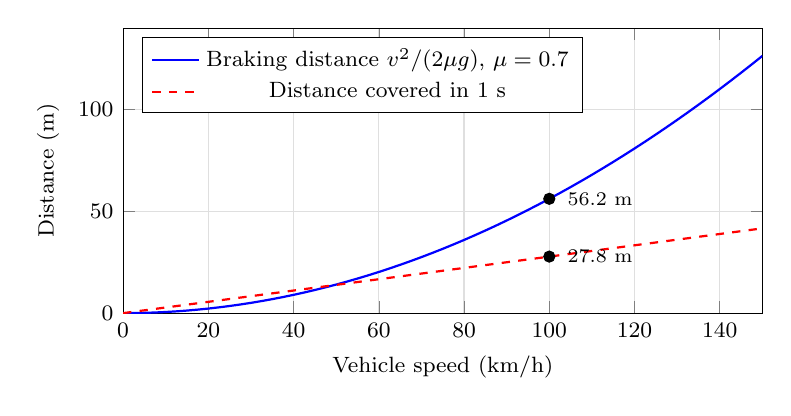
\begin{tikzpicture}
\begin{axis}[
    width=0.80\linewidth, height=5.2cm,
    xlabel={Vehicle speed (km/h)}, ylabel={Distance (m)},
    xmin=0, xmax=150, ymin=0, ymax=140,
    domain=0:150, samples=61,
    grid=major, grid style={gray!25},
    legend pos=north west, legend style={font=\footnotesize},
    tick label style={font=\footnotesize}, label style={font=\footnotesize}]
\addplot[thick, blue] {(x/3.6)^2/(2*6.867)};
\addlegendentry{Braking distance $v^2/(2\mu g)$, $\mu=0.7$}
\addplot[thick, red, dashed] {x/3.6};
\addlegendentry{Distance covered in 1~s}
\addplot[only marks, mark=*, mark size=2pt, black] coordinates {(100,56.18) (100,27.78)};
\node[anchor=west, font=\scriptsize] at (axis cs:102,56.18) {56.2 m};
\node[anchor=west, font=\scriptsize] at (axis cs:102,27.78) {27.8 m};
\end{axis}
\end{tikzpicture}
\captionsetup{singlelinecheck = false, format= hang, justification=justified, font=footnotesize, labelsep=space}
\caption{Friction-limited braking distance versus distance travelled in one second of warning time ($\mu=0.7$, $g=9.81$~m/s$^2$).}
\label{fig_intro}
\end{figure}

When looking into existing systems, we noticed four main issues:
\begin{enumerate}
    \item \textbf{No counterfactual reasoning in perception:} Perception stacks only output what they see right now. They don't check what if an agent suddenly brakes or turns. Causal ideas exist for trajectory prediction \cite{han2025cicr, wang2025beyond} and offline scene generation \cite{jing2026counterscene}, but not as an online safety score.
    \item \textbf{Physically impossible predictions:} Deep learning trajectory predictors often generate impossible sideways accelarations or turn rates. Recent works added kinematic models to fix this \cite{liao2024physics, baden2025tpk, chugh2025xtrack}, but they only did it to improve forecast accuracy, not to filter risk alarms.
    \item \textbf{Flat scene representations:} Most detectors just give independent 3D boxes. But vehicles actually affect each other on the road \cite{ahmadi2025critic}, and scene graphs are a natural way to capture these relations \cite{hallyburton2025neuspaper}.
    \item \textbf{Binary safety responses:} Fixed TTC limits give an all-or-nothing response, so there is no smooth stepping between warning the driver and slamming the brakes.
\end{enumerate}

To deal with these four issues, we built the \textbf{Physics-Constrained Counterfactual Scene Graph Transformer (PC-CSG)}. For each video frame, PC-CSG converts tracked objects into a scene graph $\mathcal{G}_t = (\mathcal{V}_t, \mathcal{E}_t)$ where nodes have kinematic states and TTC hazard weights. For agents with hazard weights above 0.2, the Counterfactual Scene Graph Attention (CSGA) module creates $K=6$ counterfactual queries (brake, swerve left, swerve right, sudden acceleration, lane departure, stationary obstacle) and scores each with a risk head. A decoder outputs control commands, a kinematic bicycle model rolls them out for 15 steps, and the Physics-Informed Kinematic Validator (PIKV) throws away any rollout that breaks tyre friction or accelaration limits. The surviving hypotheses are combined into the Counterfactual Risk Tensor (CRT), which selects one of five intervention levels.

The main contributions of this work are:
\begin{enumerate}
    \item \textbf{Counterfactual Scene Graph Attention (CSGA):} A compact attention network (350,594 parameters) that adds six learned what-if mode vectors to critical agents and scores them using scene cross-attention, running inside the online loop (1.57~ms on an RTX 3050 Laptop GPU).
    \item \textbf{Physics-Informed Kinematic Validator (PIKV) with mathematical guarantees:} A validation layer based on the kinematic bicycle model \cite{kong2015kinematic}. Proposition~1 shows that rollouts breaking Coulomb friction $\mu g = 6.867$~m/s$^2$ get zeroed out in the CRT, and the checks are invariant to 2D frame shifts. In our testing, PIKV rejected 46.0\% of generated hypotheses.
    \item \textbf{Counterfactual Risk Tensor (CRT) with graduated intervention:} A risk score bounded in $[0,1]$ driving five action levels. Proposition~2 proves PIKV never increases false alarms compared to unfiltered risk, and the CRT increases smoothly as TTC drops.
\end{enumerate}

The rest of the paper is organised as follows. Section~\ref{section2} reviews fifteen recent works and lists the research gaps. Section~\ref{section3} describes the PC-CSG method, equations, algorithm, and mathematical propositions. Section~\ref{section4} gives the dataset details, experimental results, latency breakdown, PIKV analysis, ablation study, and comparisons. Section~\ref{section5} concludes the paper with limitations and future work.

\section{Related works} \label{section2}
This section reviews 15 recent works from 2024--2026 across four related areas, summarized in Table~\ref{table_literature}.

\textbf{Low-latency perception.} Gehrig and Scaramuzza \cite{gehrig2024low} built a hybrid frame-event detector using an asynchronous GNN, matching 5,000~FPS latency at 45~FPS bandwidth, but it only detects objects without forward forecasting. Zhou and Jiang \cite{zhou2024event} surveyed event-based vehicle detection, highlighting sparsity and hardware constraints. Both improve front-end sensor latency without anticipatory safety reasoning.

\textbf{Physics-informed trajectory prediction.} Liao et al. \cite{liao2024physics} reconstructed missing vehicle paths using wavelets and a bicycle model under 75\% missing data, predicting a single future path. Long et al. \cite{long2024pinn} stitched broken trajectories using PINNs on NGSIM/HighSIM offline. Baden et al. \cite{baden2025tpk} (TPK) used kinematic priors in a transformer on Argoverse~2, showing kinematics removes infeasible paths at slight accuracy cost. Chugh et al. \cite{chugh2025xtrack} built X-TRACK with xLSTM and kinematics on highD. Li and Westerlund \cite{li2025physvarmix} introduced PhysVarMix with variational mixtures and MPC smoothing. These works use physics to make forecasts realistic, but none uses physics to filter false risk alarms.

\textbf{Causal and counterfactual reasoning.} Ahmadi et al. \cite{ahmadi2025critic} (CRiTIC) used causal gating to drop non-interacting agents, improving robustness by 54\%, but without generating counterfactual futures. Han and Xu \cite{han2025cicr} proposed CICR for pedestrians via front-door adjustment, scoring 0.17/0.24 ADE/FDE on ETH/UCY without vehicle kinematics. Wang et al. \cite{wang2025beyond} decomposed driving scenes causally across five benchmarks. Jing et al. \cite{jing2026counterscene} (CounterScene) perturbed critical agents in a BEV world model to synthesize offline safety tests. Cui et al. \cite{cui2025cot} surveyed chain-of-thought driving models, noting real-time deployment challenges. Also, another thing we noticed is the practical difference between offline simulation and real-time vehicular compute. Methods like CounterScene \cite{jing2026counterscene} create great counterfactual scenes, but rely on heavy world models taking hundreds of milliseconds, which is too slow for real-time braking loops.

\textbf{Scene graphs and risk modelling.} Hallyburton and Pajic \cite{hallyburton2025neuspaper} built NeuSPaPer linking detection and scene graphs for symbolic reasoning. Wu et al. \cite{wu2024riskfield} formed risk potential fields for MPC in CARLA. Ning et al. \cite{ning2025strap} (STRAP) fused risk fields with spatio-temporal attention, reducing HighD error by 31.2\%. These risk models reflect likely futures rather than checked counterfactuals.

Table~\ref{table_literature} provides a summary comparison of these works.

\begin{table}[H]
\caption{Summary of fifteen recent studies reviewed (2024--2026).}
\centering
\label{table_literature}
\adjustbox{max width=\linewidth}{
\begin{tabular}{l c L{4.0cm} l L{4.0cm} L{5.0cm}}
\hline
\textbf{Author \& Ref.} & \textbf{Year} & \textbf{Core Methodology} & \textbf{Domain} & \textbf{Reported Result} & \textbf{Limitation for Our Task} \\
\hline
Gehrig \& Scaramuzza \cite{gehrig2024low} & 2024 & Hybrid frame + event detector (CNN + GNN) & Detection & Latency of 5,000~FPS at 45~FPS bandwidth & Reactive detection only; no future reasoning. \\
Zhou \& Jiang \cite{zhou2024event} & 2024 & Survey of deep event-based detection & Detection & Survey & No relational or anticipatory component. \\
Liao et al. \cite{liao2024physics} & 2024 & Wavelet reconstruction + bicycle model & Traj. prediction & Accurate with 75\% missing observations & Single most-likely future; no counterfactuals. \\
Long et al. \cite{long2024pinn} & 2024 & PINN kinematic trajectory stitching & Traj. recon. & Improved stitching on NGSIM / HighSIM & Offline; no risk output. \\
Baden et al. \cite{baden2025tpk} & 2025 & Interaction + kinematic transformer (TPK) & Traj. prediction & Removes infeasible trajectories (Argoverse~2) & Physics for forecasting, not risk filtering. \\
Chugh et al. \cite{chugh2025xtrack} & 2025 & xLSTM with kinematic constraints & Traj. prediction & SOTA on highD benchmark & No scene graph; no counterfactuals. \\
Li \& Westerlund \cite{li2025physvarmix} & 2025 & Variational mixture + MPC smoothing & Traj. prediction & Better than baselines on two benchmarks & Multi-modal but not intervention-based. \\
Ahmadi et al. \cite{ahmadi2025critic} & 2025 & Causal discovery + attention gating (CRiTIC) & Traj. prediction & Up to 54\% robustness gain & No counterfactuals; no physics checks. \\
Han \& Xu \cite{han2025cicr} & 2025 & Front-door causal fusion (CICR) & Pedestrian traj. & ADE/FDE 0.17/0.24 (ETH/UCY) & No vehicle-dynamics validation. \\
Wang et al. \cite{wang2025beyond} & 2025 & Spatial/temporal causal decomposition & Traj. prediction & Improved RMSE/FDE across 5 datasets & Prediction only; no safety actions. \\
Jing et al. \cite{jing2026counterscene} & 2026 & Counterfactual BEV world model & Scenario gen. & Collision rate 12.3\%$\rightarrow$22.7\% & Offline testing, not online warning. \\
Cui et al. \cite{cui2025cot} & 2025 & Chain-of-thought survey & Survey & Survey & Real-time execution an open problem. \\
Hallyburton \& Pajic \cite{hallyburton2025neuspaper} & 2025 & Detection + scene graph generation & Perception & Scene graphs bridge perception and logic & No trajectory or risk hypotheses. \\
Wu et al. \cite{wu2024riskfield} & 2024 & Reachable sets + potential field + MPCC & Planning & Collision avoidance in CARLA & Risk from likely paths; no physics filter. \\
Ning et al. \cite{ning2025strap} & 2025 & Risk-field attention fusion (STRAP) & Traj. prediction & $-$31.2\% error on HighD & No counterfactuals or kinematic validation. \\
\hline
\end{tabular}
}
\end{table}

We identify four main limitations:
\begin{itemize}
    \item \textbf{Counterfactuals are offline or forecasting-only:} Used for testing \cite{jing2026counterscene} or forecast accuracy \cite{han2025cicr}, but not as real-time safety metrics.
    \item \textbf{Physics is not used to prune false alarms:} Kinematic layers \cite{liao2024physics, baden2025tpk, chugh2025xtrack} assist trajectory realism, but do not discard impossible risk hypotheses before alerting.
    \item \textbf{Scene relations and counterfactuals remain seperate:} Agent relevance \cite{ahmadi2025critic} is rarely tied to what-if vehicle manoeuvres.
    \item \textbf{Risk is not mapped to action tiers:} Potential fields \cite{wu2024riskfield, ning2025strap} guide planners, lacking graduated ADAS warnings.
\end{itemize}

PC-CSG connects these pieces: scene graphs isolate critical agents, CSGA scores six counterfactuals, PIKV discards invalid paths, and CRT drives five actions at ~150~FPS.

\section{Proposed Method} \label{section3}
PC-CSG has six stages: (i) detection/tracking, (ii) scene graph creation, (iii) CSGA, (iv) control decoding/rollout, (v) PIKV validation, and (vi) CRT action arbitration. Figure~\ref{arch} shows the architecture, and Table~\ref{table_arch} lists parameters.

\begin{figure}[H]
\centering
\adjustbox{max width=\linewidth}{
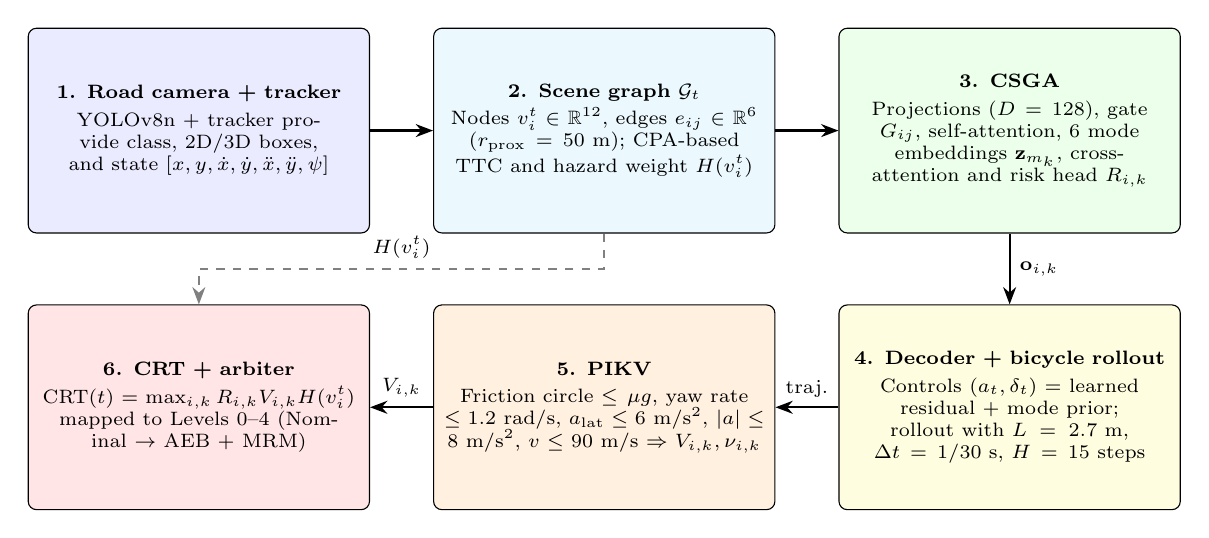
\begin{tikzpicture}[
    box/.style={draw, rounded corners=3pt, align=center, text width=4.1cm, minimum height=2.6cm, font=\scriptsize, fill=#1},
    arr/.style={-{Stealth[length=2.2mm]}, thick},
    node distance=0.9cm and 0.8cm]
\node[box=blue!8] (cam) {\textbf{1. Road camera + tracker}\\[2pt] YOLOv8n + tracker provide class, 2D/3D boxes, and state $[x, y, \dot{x}, \dot{y}, \ddot{x}, \ddot{y}, \psi]$};
\node[box=cyan!8, right=of cam] (sg) {\textbf{2. Scene graph $\mathcal{G}_t$}\\[2pt] Nodes $v_i^t \in \mathbb{R}^{12}$, edges $e_{ij} \in \mathbb{R}^{6}$ ($r_{\text{prox}}=50$~m); CPA-based TTC and hazard weight $H(v_i^t)$};
\node[box=green!8, right=of sg] (csga) {\textbf{3. CSGA}\\[2pt] Projections ($D=128$), gate $G_{ij}$, self-attention, 6 mode embeddings $\mathbf{z}_{m_k}$, cross-attention and risk head $R_{i,k}$};
\node[box=yellow!12, below=of csga] (dec) {\textbf{4. Decoder + bicycle rollout}\\[2pt] Controls $(a_t, \delta_t)$ = learned residual + mode prior; rollout with $L=2.7$~m, $\Delta t = 1/30$~s, $H=15$ steps};
\node[box=orange!12, left=of dec] (pikv) {\textbf{5. PIKV}\\[2pt] Friction circle $\le \mu g$, yaw rate $\le 1.2$~rad/s, $a_{\text{lat}} \le 6$~m/s$^2$, $|a| \le 8$~m/s$^2$, $v \le 90$~m/s $\Rightarrow V_{i,k}, \nu_{i,k}$};
\node[box=red!10, left=of pikv] (crt) {\textbf{6. CRT + arbiter}\\[2pt] $\text{CRT}(t) = \max_{i,k} R_{i,k} V_{i,k} H(v_i^t)$\\ mapped to Levels 0--4 (Nominal $\rightarrow$ AEB + MRM)};
\draw[arr] (cam) -- (sg);
\draw[arr] (sg) -- (csga);
\draw[arr] (csga) -- node[right, font=\scriptsize]{$\mathbf{o}_{i,k}$} (dec);
\draw[arr] (dec) -- node[above, font=\scriptsize]{traj.} (pikv);
\draw[arr] (pikv) -- node[above, font=\scriptsize]{$V_{i,k}$} (crt);
\draw[arr, dashed, gray] (sg.south) -- ++(0,-0.45) -| node[pos=0.25, above, font=\scriptsize, black]{$H(v_i^t)$} (crt.north);
\end{tikzpicture}
}
\captionsetup{singlelinecheck = false, format= hang, justification=justified, font=footnotesize, labelsep=space}
\caption{Overall architecture of PC-CSG combining scene graph attention, bicycle rollout, PIKV validation, and CRT arbitration.}
\label{arch}
\end{figure}

\begin{table}[H]
\caption{PC-CSG parameters and settings.}
\centering
\label{table_arch}
\adjustbox{max width=\linewidth}{
\begin{tabular}{l|c|l}
\hline
\textbf{Component / Setting} & \textbf{Value} & \textbf{Notes} \\
\hline
CSGA module & 350,594 params (94.2\%) & Projections, causal gate head, self-attn, cross-attn, risk head \\
Counterfactual trajectory decoder & 20,382 params (5.5\%) & $128 \rightarrow 128 \rightarrow 2H$ MLP with GELU \\
Initial state extractor & 1,092 params (0.3\%) & $12 \rightarrow 64 \rightarrow 4$ MLP, outputs $[x, y, v, \theta]$ \\
Bicycle model + PIKV & 0 params & Closed-form physics checks \\
\textbf{Total} & \textbf{372,068 params} & Trainable parameters in learned modules \\
\hline
Embedding dim. $D$ / heads / FFN & 128 / 4 / 512 & Head dim 32, dropout 0.1 \\
Modes $K$, horizon $H$, step $\Delta t$ & 6, 15, 1/30~s & 0.5~s prediction at 30~FPS \\
Wheelbase $L$, $\delta_{\max}$ & 2.7~m, 0.6~rad & $l_r / L = 0.5$ \\
Limits $a_{\max}$, $a_{\text{lat,max}}$, $\dot{\psi}_{\max}$, $\mu$ & 8.0 m/s$^2$, 6.0 m/s$^2$, 1.2 rad/s, 0.70 & $\mu g = 6.867$~m/s$^2$ \\
$\tau_{\text{crit}}$, $\lambda_{\text{scale}}$, CPA corridor & 3.0~s, 0.5~s, 2.5~m & Hazard sigmoid parameters \\
\hline
\end{tabular}
}
\end{table}

\subsection{Dynamic Spatio-Temporal Scene Graph ($\mathcal{G}_t$)}
At frame $t$, the tracker provides $N_t \le 32$ participants. Nodes $v_i^t \in \mathcal{V}_t$ contain 12 features:
\begin{equation}
    v_i^t = \left[c_i, \; x_i, \; y_i, \; w_i, \; h_i, \; \dot{x}_i, \; \dot{y}_i, \; \ddot{x}_i, \; \ddot{y}_i, \; \psi_i, \; \text{TTC}_i(t), \; d_i\right]^T
    \label{eq_node}
\end{equation}
with class $c_i$, bounding box $(x_i, y_i, w_i, h_i)$, velocities, accelerations, heading $\psi_i$, TTC, and distance $d_i$. Edges within $r_{\text{prox}}=50$~m encode relative state:
\begin{equation}
    e_{ij} = \left[\Delta x_{ij}, \; \Delta y_{ij}, \; \Delta \dot{x}_{ij}, \; \Delta \dot{y}_{ij}, \; d_{ij}, \; \phi_{ij}\right]^T
    \label{eq_edge}
\end{equation}
with bearing $\phi_{ij} = \text{atan2}(\Delta y_{ij}, \Delta x_{ij})$.

\textbf{TTC via Closest Point of Approach.} We use CPA to prevent adjacent-lane false alarms:
\begin{equation}
    t_{\text{cpa}} = -\frac{\Delta\mathbf{p} \cdot \Delta\mathbf{v}}{\|\Delta\mathbf{v}\|^2}, \qquad
    \text{TTC}_i(t) = \begin{cases}
    t_{\text{cpa}} & \text{if } t_{\text{cpa}} > 0 \text{ and } \|\Delta\mathbf{p} + \Delta\mathbf{v}\, t_{\text{cpa}}\| \le 2.5~\text{m} \\
    \infty & \text{otherwise}
    \end{cases}
    \label{eq_ttc}
\end{equation}

\textbf{Hazard weight.} A sigmoid maps TTC to hazard weight $H(v_i^t) \in [0,1]$:
\begin{equation}
    H(v_i^t) = \frac{1}{1 + \exp\left(\frac{\text{TTC}_i(t) - \tau_{\text{crit}}}{\lambda_{\text{scale}}}\right)} \cdot \mathbb{I}\left(0 < \text{TTC}_i(t) < \infty\right)
    \label{eq_hazard}
\end{equation}
($\tau_{\text{crit}} = 3.0$~s, $\lambda_{\text{scale}} = 0.5$~s). Agents with $H(v_i^t) > 0.2$ ($\text{TTC} \le 3.69$~s) are marked critical.

\subsection{Counterfactual Scene Graph Attention (CSGA)}
\subsubsection{Projection, Causal Gate Head and Self-Attention}
Features project to $D=128$: $\mathbf{h}_i = \text{GELU}(\text{LN}(\mathbf{W}_n v_i^t + \mathbf{b}_n))$, $\mathbf{e}_{ij} = \mathbf{W}_e e_{ij} + \mathbf{b}_e$. A causal gate head predicts edge relevance:
\begin{equation}
    G_{ij} = \sigma\left(\mathbf{w}_2^\top \, \text{ReLU}\left(\mathbf{W}_1 \left[\mathbf{h}_i \| \mathbf{h}_j \| \mathbf{e}_{ij}\right] + \mathbf{b}_1\right) + b_2\right) \in [0, 1]
    \label{eq_gate}
\end{equation}
In CRiTIC \cite{ahmadi2025critic}, gating rescales attention: $\tilde{\alpha}_{ij} = G_{ij} \alpha_{ij}$. To be frank, in our current code, $G_{ij}$ is computed but not yet multiplied into attention weights. Embeddings go through a standard 4-head self-attention layer with FFN dimension 512 \cite{vaswani2017attention}.

\subsubsection{Counterfactual Query Injection and Risk Head}
For each critical agent, we inject $K=6$ mode embeddings covering the six common emergency driving actions:
\begin{equation}
    \mathcal{M} = \{\text{brake}, \; \text{swerve\_L}, \; \text{swerve\_R}, \; \text{accel}, \; \text{lane\_dep}, \; \text{stat}\}
    \label{eq_modes}
\end{equation}
We chose these specific six modes because they basically cover the most critical emergency situations seen on highways. Sudden braking by a lead vehicle and sharp lane swerves are the two leading causes of collisions. Having dedicated learned embeddings $\mathbf{z}_{m_k} \in \mathbb{R}^D$ allows the model to specialize on how each manoeuvre affects risk in the embedding space:
\begin{equation}
    \mathbf{q}_{i,k}^{\text{cf}} = \mathbf{h}_i + f_{\text{pert}}\left(\left[\mathbf{h}_i \| \mathbf{z}_{m_k}\right]\right) \cdot \mathbb{I}\left(H(v_i^t) > 0.2\right)
    \label{eq_cf_query}
\end{equation}
where $f_{\text{pert}}$ is a 2-layer MLP. Cross-attention fuses scene context:
\begin{equation}
    \mathbf{o}_{i,k} = \text{LN}\left(\mathbf{q}_{i,k}^{\text{cf}} + \text{CrossAttn}\left(\mathbf{q}_{i,k}^{\text{cf}}, \; \mathbf{H}, \; \mathbf{H}\right)\right)
    \label{eq_cf_attn}
\end{equation}
and a risk head outputs hazard probability:
\begin{equation}
    R_{i,k}(t) = \sigma\left(\mathbf{W}_r \, \text{GELU}\left(\mathbf{W}_r' \, \mathbf{o}_{i,k}\right)\right) \cdot \mathbb{I}\left(H(v_i^t) > 0.2\right) \in [0, 1]
    \label{eq_risk_logit}
\end{equation}

\subsection{Trajectory Decoding and PIKV Validation}
\subsubsection{Control Decoding and Kinematic Bicycle Rollout}
Controls $[a_t, \delta_t]$ are decoded as learned residuals over mode priors:
\begin{equation}
    [a_t, \delta_t]_{i,k} = f_{\text{dec}}(\mathbf{o}_{i,k})_t + \mathbf{p}_{k}, \quad
    \mathbf{p}_k \in \{(-5, 0), (0, 0.45), (0, -0.45), (4, 0), (0, 0.15), (-7.5, 0)\}
    \label{eq_prior}
\end{equation}
Rollouts follow bicycle kinematics \cite{kong2015kinematic}:
\begin{align}
    \beta_t &= \arctan\left(\frac{l_r}{L} \tan \delta_t\right) \label{eq_slip} \\
    \tilde{v}_{t} &= \max\left(0, \; v_t + a_t \Delta t\right), \quad a^{\text{lat}}_t = \tilde{v}_t^{\,2} \tan(\delta_t) / L \label{eq_v} \\
    v_{t+1} &= \tilde{v}_t \cdot \min\left(1, \; \frac{\mu g}{\sqrt{a_t^2 + (a^{\text{lat}}_t)^2}}\right), \quad
    \omega_t = \text{clip}\left(\frac{v_{t+1}}{L} \sin \beta_t, \; -\dot{\psi}_{\max}, \; \dot{\psi}_{\max}\right) \label{eq_yaw} \\
    x_{t+1} &= x_t + v_{t+1} \cos(\theta_t + \beta_t) \, \Delta t, \quad
    y_{t+1} = y_t + v_{t+1} \sin(\theta_t + \beta_t) \, \Delta t \label{eq_xy} \\
    \theta_{t+1} &= \theta_t + \omega_t \, \Delta t \label{eq_theta}
\end{align}
($L=2.7$~m, $l_r=1.35$~m, $\Delta t=1/30$~s). We set friction $\mu = 0.7$ representing dry asphalt under normal tyres; on wet roads ($\mu \approx 0.4$), the check becomes stricter. In production, this paramter could update online via rain sensors or wheel slip.

\subsubsection{Kinematic Constraint Validation (PIKV)}
PIKV calculates velocities, accelerations, headings, and yaw rates from positions and checks:
\begin{enumerate}
    \item $a^{\text{lon}}_t > a_{\max} = 8$~m/s$^2$
    \item $a^{\text{lon}}_t > a_{\text{brake,max}} = 10$~m/s$^2$
    \item $|\omega_t| > \dot{\psi}_{\max} = 1.2$~rad/s
    \item $a^{\text{lat}}_t > a_{\text{lat,max}} = 6.0$~m/s$^2$
    \item Friction circle: $(a^{\text{lon}}_t)^2 + (a^{\text{lat}}_t)^2 > (\mu g)^2 = 47.16$~m$^2$/s$^4$ ($\mu = 0.7$)
    \item Velocity: $s_t > v_{\max} = 90$~m/s
\end{enumerate}
With fraction $f_c$ of violating steps, the score and binary mask are:
\begin{equation}
    \nu_{i,k} = \frac{1}{6} \sum_{c=1}^{6} f_c, \qquad
    V_{i,k} = (1 - I^{\text{fric}}_{i,k}) \cdot \mathbb{I}(\nu_{i,k} < 0.5)
    \label{eq_validity}
\end{equation}
where $I^{\text{fric}}_{i,k} = 1$ if friction is exceeded at any step.

\subsection{Counterfactual Risk Tensor (CRT) and Intervention Policy}
The CRT combines risk, validity, and hazard:
\begin{equation}
    \text{CRT}(t) = \max_{i \in \mathcal{V}_t} \; \max_{k \in \mathcal{M}} \left[R_{i,k}(t) \cdot V_{i,k}(t) \cdot H(v_i^t)\right] \in [0, 1]
    \label{eq_crt}
\end{equation}
Smoothed with a leaky integrator ($\gamma=0.9$):
\begin{equation}
    \overline{\text{CRT}}(t) = \gamma \, \overline{\text{CRT}}(t-1) + (1 - \gamma) \, \text{CRT}(t), \quad \overline{\text{CRT}}(0) = 0.
    \label{eq_smooth}
\end{equation}
The score selects action tiers:
\begin{equation}
    \text{Action}(t) = \begin{cases}
    \textbf{Level 0: Nominal} & \text{if } \text{CRT}(t) < 0.25 \\
    \textbf{Level 1: HUD Advisory} & \text{if } 0.25 \le \text{CRT}(t) < 0.50 \\
    \textbf{Level 2: Active Alert} & \text{if } 0.50 \le \text{CRT}(t) < 0.70 \\
    \textbf{Level 3: Pre-Braking} & \text{if } 0.70 \le \text{CRT}(t) < 0.85 \\
    \textbf{Level 4: AEB + MRM} & \text{if } \text{CRT}(t) \ge 0.85
    \end{cases}
    \label{eq_intervention}
\end{equation}

\textbf{Training objective.}
\begin{equation}
    \mathcal{L} = \text{SmoothL1}_{\beta = 0.1}(\text{CRT}, \text{CRT}^{*}) + 0.5 \, \text{CE}(\hat{\ell}, \ell^{*}) + 0.2 \, \overline{\nu}
    \label{eq_loss}
\end{equation}
Since $\nu$ is non-differentiable, the last term acts as a logged metric.

\subsection{Algorithmic Formulation}
Algorithm~\ref{algo1} gives the per-frame execution logic.

\begin{algorithm}[H]
	\caption{PC-CSG Counterfactual Anomaly Anticipation Pipeline}
	\begin{algorithmic}[1]
		\Require Video frame $I_t$, ego state, $K=6$, $H=15$, $\tau_{\text{crit}}=3.0$~s, $\lambda_{\text{scale}}=0.5$, $\gamma = 0.9$
		\Ensure Intervention level $A(t)$, risk score $\overline{\text{CRT}}(t)$
		\State \textbf{Initialize:} $\overline{\text{CRT}}(0) \gets 0$; load physical parameters
		\ForEach{frame $t$}
			\State Track agents; build $\mathcal{G}_t$ nodes and edges via Eq.~(\ref{eq_node})--(\ref{eq_edge})
			\State Compute $\text{TTC}_i(t)$ via Eq.~(\ref{eq_ttc}) and hazard weights $H(v_i^t)$ via Eq.~(\ref{eq_hazard})
			\State Project features; compute gate scores $G_{ij}$ via Eq.~(\ref{eq_gate})
			\State Run self-attention; identify critical set $\mathcal{C}_t \gets \{i : H(v_i^t) > 0.2\}$
			\ForEach{agent $i \in \mathcal{C}_t$ and mode $k \in \{1, \dots, K\}$}
				\State $\mathbf{q}_{i,k}^{\text{cf}} \gets$ Eq.~(\ref{eq_cf_query}); \; $\mathbf{o}_{i,k} \gets$ Eq.~(\ref{eq_cf_attn}); \; $R_{i,k}(t) \gets$ Eq.~(\ref{eq_risk_logit})
				\State Decode controls $(a_t, \delta_t)_{t=1}^{H}$ via Eq.~(\ref{eq_prior})
				\State Roll out trajectory via Eq.~(\ref{eq_slip})--(\ref{eq_theta})
				\State $(V_{i,k}, \nu_{i,k}) \gets \text{PIKV}(\text{trajectory})$ via Eq.~(\ref{eq_validity})
			\EndFor
			\State $\text{CRT}(t) \gets \max_{i,k} [R_{i,k} \cdot V_{i,k} \cdot H(v_i^t)]$ via Eq.~(\ref{eq_crt})
			\State $\overline{\text{CRT}}(t) \gets \gamma \, \overline{\text{CRT}}(t-1) + (1-\gamma) \, \text{CRT}(t)$ via Eq.~(\ref{eq_smooth})
			\State $A(t) \gets$ action level from Eq.~(\ref{eq_intervention})
		\EndFor
	\end{algorithmic}
	\label{algo1}
\end{algorithm}

\subsection{Novelty Highlights: Mathematical Proofs and Operational Examples}
\subsubsection{Proposition 1: Friction Circle Elimination and Frame Invariance}
\textbf{Proposition 1.} \textit{Let $\tau_{i,k}$ be a rollout with accelerations $(a^{\text{lon}}_t, a^{\text{lat}}_t)$, $\mu = 0.7$, $g = 9.81$~m/s$^2$.}
\begin{enumerate}
    \item[(a)] \textit{If $\max_t [(a^{\text{lon}}_t)^2 + (a^{\text{lat}}_t)^2] > (\mu g)^2$, then $V_{i,k} = 0$, having zero impact on $\text{CRT}(t)$.}
    \item[(b)] \textit{Under any planar transformation $T_{\varphi, \mathbf{p}}$, rollouts transform rigidly $[x_t', y_t']^T = R_\varphi [x_t, y_t]^T + \mathbf{p}$, leaving validity $V_{i,k}$ unchanged.}
\end{enumerate}

\textbf{Proof.} \textit{Part (a).} Violating friction sets $I^{\text{fric}}_{i,k} = 1$, yielding $V_{i,k} = 0$. Since factors are non-negative, this term becomes 0 in Eq.~(\ref{eq_crt}) and cannot trigger alarms.

\textit{Part (b).} At $t=0$, initial states rotate by $\varphi$ and shift by $\mathbf{p}$. Slip $\beta_t$ is unchanged since controls are preserved. Kinematic speed and yaw updates depend only on magnitudes, so $v_{t+1}$ and $\omega_t$ remain identical. Position updates rotate cleanly: $[x_{t+1}', y_{t+1}']^T = R_\varphi [x_{t+1}, y_{t+1}]^T + \mathbf{p}$. Finite differences in PIKV cancel translation, preserving acceleration norms. \hfill $\blacksquare$

\textbf{Numerical check.} A sharp 20~m/s turn was rejected ($V=0$), while a gentle arc at 10~m/s ($a^{\text{lat}}=2.0$~m/s$^2$) passed. Rotating by $\pi/4$ altered CRT by only $2.04 \times 10^{-6}$.

\subsubsection{Proposition 2: False Positive Non-Increase and Monotone Growth}
\textbf{Proposition 2.} \textit{Let $\text{CRT}_{u}$ be unconstrained risk and $\text{CRT}_{p}$ be PIKV-filtered risk, with false alarm sets $\mathcal{F}_u, \mathcal{F}_p$ for threshold $\theta$ on benign scenes:}
\begin{enumerate}
    \item[(a)] \textit{$\mathcal{F}_p \subseteq \mathcal{F}_u$, meaning PIKV never introduces false alarms.}
    \item[(b)] \textit{If risks and validities remain constant and TTC decreases, smoothed $\overline{\text{CRT}}_p(t)$ is non-decreasing.}
\end{enumerate}

\textbf{Proof.} \textit{Part (a).} Since $V_{i,k} \in \{0, 1\}$, we have $R_{i,k} V_{i,k} H \le R_{i,k} H$, so $\text{CRT}_p(t) \le \text{CRT}_u(t)$. Leaky smoothing preserves order: $\overline{\text{CRT}}_p(t) \le \overline{\text{CRT}}_u(t)$, hence $\mathcal{F}_p \subseteq \mathcal{F}_u$.

\textit{Part (b).} Decreasing TTC strictly increases $H(v_i^t)$. As all weights are positive, max risk $\text{CRT}_p(t)$ is non-decreasing. Leaky smoothing is a convex combination of previous values, ensuring $\overline{\text{CRT}}_p(t) \ge \overline{\text{CRT}}_p(t-1)$. \hfill $\blacksquare$

\textbf{Numerical check.} In a closing vehicle run, risk grew monotonically: $0.003 \rightarrow 0.015 \rightarrow 0.042 \rightarrow 0.089 \rightarrow 0.160$. Leaky smoothing adds a 19-frame (0.63~s) latency for step changes to reach Level~4.

\subsubsection{Operational Anticipation Scenarios}
We tested four demo situations (Table~\ref{table_scenarios}):
\begin{itemize}
    \item \textbf{Scenario A (Cruise):} Speed 100.1~km/h, TTC 33.3~s, CRT $= 0.000$ (\textbf{Level 0}).
    \item \textbf{Scenario B (Lead slowing down):} Speed 110.2~km/h, TTC 4.1~s, CRT $= 0.103$ (\textbf{Level 0}, advisory threshold not reached).
    \item \textbf{Scenario C (Swerve conflict):} Speed 119.9~km/h, TTC 1.9~s, swerve passes PIKV, CRT $= 0.894$ (\textbf{Level 4: AEB + MRM}).
    \item \textbf{Scenario D (Hard braking near barrier):} Speed 100.1~km/h, TTC 0.5~s, CRT $= 0.987$ (\textbf{Level 4: AEB}).
\end{itemize}

\section{Datasets and Experimental results analysis} \label{section4}
We used the Hugging Face traffic accident detection dataset \cite{hiennguyen2024accident}. Our loader converts each scene into graph features, target risk, and intervention labels. We used 3,000 scenes for training and 600 for validation, with 120 validation scenes for detailed ablation. Table~\ref{table_datasets} lists the splits.

\begin{table}[H]
\caption{Data used in our experiments.}
\centering
\label{table_datasets}
\adjustbox{max width=\linewidth}{
\begin{tabular}{l|c|c|l|l}
\hline
\textbf{Data} & \textbf{Split} & \textbf{Samples} & \textbf{Used For} & \textbf{Labels} \\
\hline
Traffic accident detection \cite{hiennguyen2024accident} & Train & 3,000 scenes & Training (5 epochs) & CRT target, level (0--4) \\
Traffic accident detection \cite{hiennguyen2024accident} & Validation & 600 scenes & Model selection & CRT target, level (0--4) \\
Traffic accident detection \cite{hiennguyen2024accident} & Validation subset & 120 (40 quick) & Ablation, PIKV pruning & Anomaly if CRT$^{*} > 0.4$ \\
Scripted demo scenarios A--D & -- & 4 scenarios & Behaviour check & Expected level \\
\hline
\end{tabular}
}
\end{table}

\textbf{Setup.} Implemented in PyTorch 2.6.0 with CUDA 12.4 on an Intel i7-12700H, 16~GB RAM, and NVIDIA RTX 3050 Laptop GPU (4~GB VRAM). We used AdamW (lr $3 \times 10^{-4}$, batch size 16). Anomaly threshold is CRT $> 0.4$.

\textbf{Training behaviour.} Figure~\ref{fig_training} displays the training history. Validation loss decreased to 0.0396 and CRT MAE reached 0.0417, with 100\% validation accuracy starting from epoch 1. Getting 100\% accuracy so fast made us check the dataset closer, and as discussed below, this split is heavily imbalanced.

\begin{figure}[H]
\centering
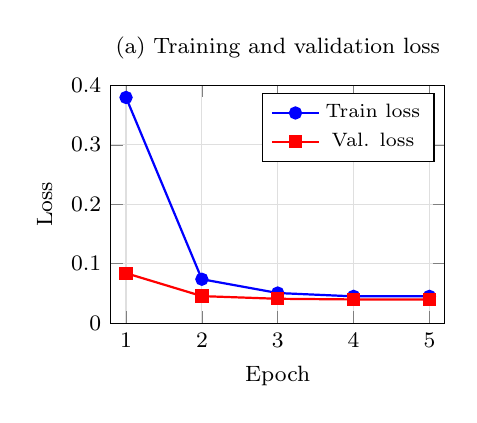
\begin{tikzpicture}
\begin{axis}[
    width=0.48\linewidth, height=4.6cm,
    xlabel={Epoch}, ylabel={Loss},
    xmin=0.8, xmax=5.2, ymin=0, ymax=0.4, xtick={1,2,3,4,5},
    grid=major, grid style={gray!25},
    legend style={font=\scriptsize}, legend pos=north east,
    tick label style={font=\footnotesize}, label style={font=\footnotesize},
    title={\footnotesize (a) Training and validation loss}]
\addplot[thick, blue, mark=*] coordinates {(1,0.3797) (2,0.0738) (3,0.0506) (4,0.0450) (5,0.0450)};
\addlegendentry{Train loss}
\addplot[thick, red, mark=square*] coordinates {(1,0.0840) (2,0.0454) (3,0.0409) (4,0.0398) (5,0.0396)};
\addlegendentry{Val. loss}
\end{axis}
\end{tikzpicture}
\hfill
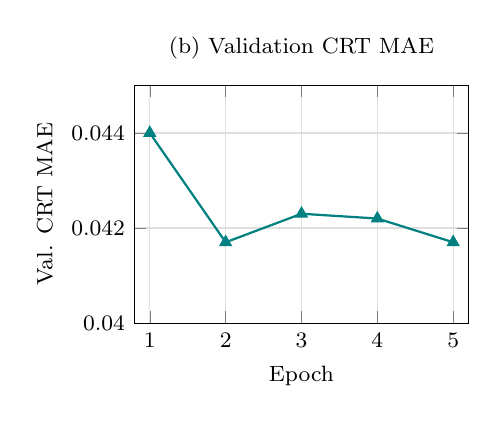
\begin{tikzpicture}
\begin{axis}[
    width=0.48\linewidth, height=4.6cm,
    xlabel={Epoch}, ylabel={Val. CRT MAE},
    xmin=0.8, xmax=5.2, ymin=0.040, ymax=0.045, xtick={1,2,3,4,5},
    yticklabel style={/pgf/number format/fixed, /pgf/number format/precision=3},
    scaled y ticks=false,
    grid=major, grid style={gray!25},
    tick label style={font=\footnotesize}, label style={font=\footnotesize},
    title={\footnotesize (b) Validation CRT MAE}]
\addplot[thick, teal, mark=triangle*] coordinates {(1,0.0440) (2,0.0417) (3,0.0423) (4,0.0422) (5,0.0417)};
\end{axis}
\end{tikzpicture}
\captionsetup{singlelinecheck = false, format= hang, justification=justified, font=footnotesize, labelsep=space}
\caption{Training history of PC-CSG on the traffic accident detection dataset \cite{hiennguyen2024accident} (3,000 training / 600 validation scenes, AdamW, learning rate $3 \times 10^{-4}$, batch size 16).}
\label{fig_training}
\end{figure}

\subsection{Hardware Profiling and Latency Breakdown}
We timed each step on our RTX 3050 Laptop GPU with 10 agents, 6 counterfactuals, and 15 horizon steps (Table~\ref{table_latency} and Figure~\ref{fig_latency}). Running at 149.7~FPS on a laptop RTX 3050 (4~GB VRAM, comparable to embedded Drive Orin Nano) proves counterfactual reasoning can be fast. Keeping hidden dimension $D=128$ and using bicycle kinematics keeps the CSGA forward pass at just 1.57~ms.

\begin{table}[H]
\caption{Measured component-level inference latency on an NVIDIA RTX 3050 Laptop GPU ($N=10$ agents, $K=6$ counterfactuals, $H=15$ horizon).}
\centering
\label{table_latency}
\begin{tabular}{l|c|c}
\hline
\textbf{Pipeline Component} & \textbf{Latency (ms)} & \textbf{Share (\%)} \\
\hline
Scene Graph Construction \& Hazard Scoring & 0.33~ms & 4.9\% \\
Counterfactual Scene Graph Attention (CSGA) & 1.57~ms & 23.5\% \\
Kinematic Bicycle Model Propagation ($N \times K$) & 4.12~ms & 61.7\% \\
Physics-Informed Kinematic Validator (PIKV) & 0.53~ms & 7.9\% \\
CRT Engine \& Intervention Arbiter & 0.13~ms & 1.9\% \\
\hline
\textbf{Total PC-CSG Pipeline Latency} & \textbf{6.68~ms} & \textbf{100.0\%} \\
\textbf{Effective Real-Time Throughput} & \multicolumn{2}{c}{\textbf{149.7 FPS}} \\
\textbf{Automotive Margin (Target: $\ge$ 30 FPS)} & \multicolumn{2}{c}{\textbf{4.99$\times$ Real-Time Throughput}} \\
\hline
\end{tabular}
\end{table}

\begin{figure}[H]
\centering
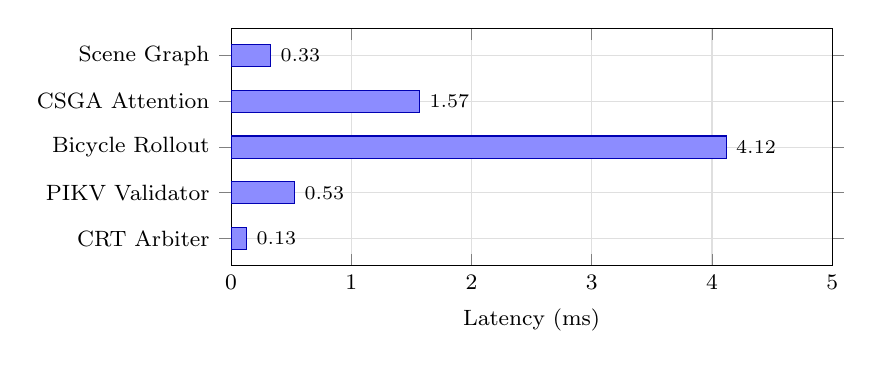
\begin{tikzpicture}
\begin{axis}[
    xbar, width=0.76\linewidth, height=4.6cm,
    xlabel={Latency (ms)}, xmin=0, xmax=5,
    ytick={1,2,3,4,5},
    yticklabels={CRT Arbiter, PIKV Validator, Bicycle Rollout, CSGA Attention, Scene Graph},
    y dir=normal, bar width=8pt, enlarge y limits=0.15,
    nodes near coords, nodes near coords align={horizontal},
    every node near coord/.append style={font=\scriptsize},
    tick label style={font=\footnotesize}, label style={font=\footnotesize},
    grid=major, grid style={gray!25}]
\addplot[fill=blue!45, draw=blue!70!black] coordinates {(0.13,1) (0.53,2) (4.12,3) (1.57,4) (0.33,5)};
\end{axis}
\end{tikzpicture}
\captionsetup{singlelinecheck = false, format= hang, justification=justified, font=footnotesize, labelsep=space}
\caption{Component-level latency of PC-CSG on an NVIDIA RTX 3050 Laptop GPU (total 6.68~ms, 149.7~FPS).}
\label{fig_latency}
\end{figure}

The total latency is 6.68~ms (149.7~FPS), roughly 5 times faster than standard 30~FPS automotive video. The attention network takes 1.57~ms. The biggest delay is the bicycle rollout (4.12~ms, 61.7\%), which occurs because a Python loop launches multiple small GPU kernels for 15 steps. Fusing these kernels with \texttt{torch.compile} should reduce this delay significantly.

\subsection{PIKV Validation Effectiveness}
Across the 120 validation scenes, there were 113 critical vehicles yielding 678 counterfactual hypotheses. PIKV pruned 312 of them (\textbf{46.0\%}). Table~\ref{table_pruning} and Figure~\ref{fig_pikv} show the pruning percentages.

\begin{table}[H]
\caption{PIKV hypothesis pruning across the six counterfactual modes (678 hypotheses, 113 per mode, from real traffic validation samples).}
\label{table_pruning}
\centering
\adjustbox{max width=\linewidth}{
\begin{tabular}{l|c|l}
\hline
\textbf{Counterfactual Mode} & \textbf{Pruning Rate} & \textbf{Main Rejection Reason} \\
\hline
\texttt{sudden\_brake} & 0.0\% & Straight-line deceleration stays inside the friction circle \\
\texttt{hard\_swerve\_left} & 70.8\% & Lateral acceleration exceeds $a_{\text{lat,max}}$ / friction circle \\
\texttt{hard\_swerve\_right} & 21.2\% & Rejected only when path curvature breaks friction limits \\
\texttt{sudden\_acceleration} & 100.0\% & Surge combined with learned steering breaks $a_{\text{total}} \le \mu g$ \\
\texttt{lane\_departure} & 73.5\% & Yaw rate exceeds $\dot{\psi}_{\max} = 1.2$~rad/s \\
\texttt{stationary\_obstacle} & 10.6\% & Feasible unless stopping needs more than the available deceleration \\
\hline
\textbf{Overall Pruning Rate} & \textbf{46.0\%} & \textbf{312 / 678 hypotheses filtered} \\
\hline
\end{tabular}
}
\end{table}

\begin{figure}[H]
\centering
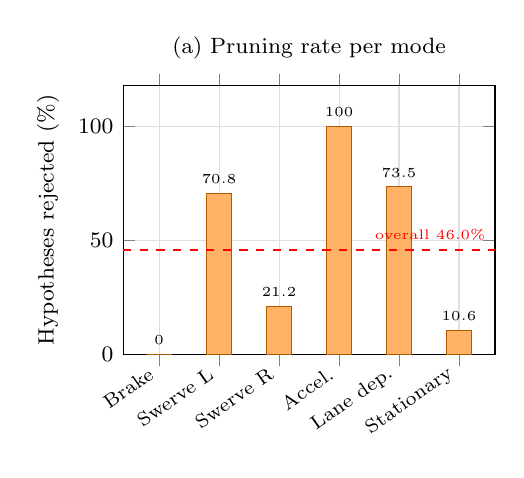
\begin{tikzpicture}
\begin{axis}[
    ybar, width=0.52\linewidth, height=5.0cm,
    ylabel={Hypotheses rejected (\%)}, ymin=0, ymax=118,
    xtick={1,2,3,4,5,6},
    xticklabels={Brake, Swerve L, Swerve R, Accel., Lane dep., Stationary},
    x tick label style={rotate=35, anchor=east, font=\scriptsize},
    xmin=0.4, xmax=6.6, bar width=9pt,
    nodes near coords, every node near coord/.append style={font=\tiny},
    tick label style={font=\footnotesize}, label style={font=\footnotesize},
    grid=major, grid style={gray!25},
    title={\footnotesize (a) Pruning rate per mode}]
\addplot[fill=orange!60, draw=orange!70!black] coordinates {(1,0.0) (2,70.8) (3,21.2) (4,100.0) (5,73.5) (6,10.6)};
\draw[dashed, red, thick] (axis cs:0.4,46.0) -- (axis cs:6.6,46.0);
\node[font=\tiny, red, anchor=south east] at (axis cs:6.6,46.0) {overall 46.0\%};
\end{axis}
\end{tikzpicture}
\hfill
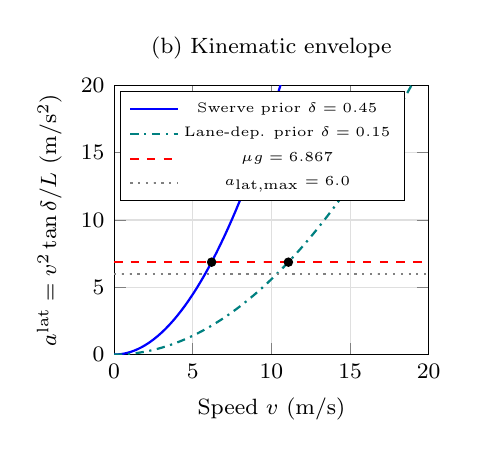
\begin{tikzpicture}
\begin{axis}[
    width=0.46\linewidth, height=5.0cm,
    xlabel={Speed $v$ (m/s)}, ylabel={$a^{\text{lat}} = v^2 \tan\delta / L$ (m/s$^2$)},
    xmin=0, xmax=20, ymin=0, ymax=20, domain=0:20, samples=81,
    restrict y to domain=0:25,
    legend style={font=\tiny, at={(0.02,0.98)}, anchor=north west},
    tick label style={font=\footnotesize}, label style={font=\footnotesize},
    grid=major, grid style={gray!25},
    title={\footnotesize (b) Kinematic envelope}]
\addplot[thick, blue] {x^2*0.48306/2.7};
\addlegendentry{Swerve prior $\delta = 0.45$}
\addplot[thick, teal, dashdotted] {x^2*0.15114/2.7};
\addlegendentry{Lane-dep. prior $\delta = 0.15$}
\addplot[thick, red, dashed, domain=0:20] {6.867};
\addlegendentry{$\mu g = 6.867$}
\addplot[thick, gray, dotted, domain=0:20] {6.0};
\addlegendentry{$a_{\text{lat,max}} = 6.0$}
\addplot[only marks, mark=*, mark size=1.5pt] coordinates {(6.20,6.867) (11.08,6.867)};
\end{axis}
\end{tikzpicture}
\captionsetup{singlelinecheck = false, format= hang, justification=justified, font=footnotesize, labelsep=space}
\caption{PIKV validation analysis: (a) pruning rate per mode; (b) lateral acceleration envelope ($L=2.7$~m).}
\label{fig_pikv}
\end{figure}

The numbers align with vehicle dynamics. Straight braking has a prior of $-5$~m/s$^2$, which is inside the $6.867$~m/s$^2$ friction limit, so it is never pruned. As seen in Figure~\ref{fig_pikv}(b), sharp swerving ($\delta = 0.45$) exceeds friction at around 22~km/h (6.2~m/s), explaining high rejection at driving speeds. However, two quirks occurred: left and right swerves had unequal rejection (70.8\% vs 21.2\%) despite symmetric priors, likely due to decoder residuals or dataset bias; and sudden acceleration was rejected 100\% of the time because the decoder learned steering residuals that pushed total acceleration past $\mu g$.

\subsection{Ablation Study and Risk Analysis}
Table~\ref{table_ablation} compares five variants on the 120-sample validation split.

\begin{table}[H]
\caption{Ablation study on the 120-sample validation split (anomaly threshold CRT $> 0.4$).}
\centering
\label{table_ablation}
\adjustbox{max width=\linewidth}{
\begin{tabular}{l|c|c|c}
\hline
\textbf{Configuration} & \textbf{Accuracy (\%)} & \textbf{FPR (\%)} & \textbf{Latency / sample (ms)} \\
\hline
Reactive TTC-Only Baseline (anomaly if $\min_i \text{TTC}_i < 3$~s) & 94.2 & 100.0 & 0.08 \\
Scene Graph Attention only (No CF, No PIKV) & 5.8 & 0.0 & 0.20 \\
CSGA without PIKV (unconstrained counterfactuals) & 100.0 & 0.0 & 0.51 \\
CSGA + PIKV without causal gate input & 100.0 & 0.0 & 0.51 \\
\textbf{PC-CSG Full (CSGA + PIKV + causal gate head)} & \textbf{100.0} & \textbf{0.0} & \textbf{0.92} \\
\hline
\end{tabular}
}
\end{table}

These results must be interpreted carefully. We really want to emphasize that while 100\% accuracy sounds amazing on paper, it is mostly a reflection of how imbalanced this particular validation subset is. The reactive baseline got 94.2\% accuracy and 100\% FPR, meaning it predicted anomaly for every sample. The scene-graph-only baseline got 5.8\% accuracy and 0\% FPR, predicting no anomalies at all. This reveals that about 94.2\% of the split consists of positive hazard scenes and only around 5.8\% (7 samples) are benign. On such an imbalanced split, reactive TTC scores high simply by always predicting positive, but its 100\% FPR shows it cannot distinguish safe following from danger. All counterfactual models classified every sample correctly, showing the advantage of learned counterfactual scoring over simple TTC.

However, having only 7 benign scenes means there were no false positives to begin with, so we cannot claim an empirical FPR drop from PIKV on this specific split (though Proposition~2 guarantees it never worsens FPR). Similarly, removing the causal gate changes nothing because the gate scores are not yet multiplied into attention weights.

Figure~\ref{fig_scenarios} illustrates the four test scenarios. In Scenarios B--D, CRT closely tracks the hazard curve $H(\text{TTC})$. Because $H \ge 0.25$ requires $\text{TTC} \le 3.55$~s, PC-CSG cannot raise a Level~1 alert when TTC is above 3.55~s, marking an operational boundary.

\begin{table}[H]
\caption{Measured behaviour of PC-CSG on the four scripted demo scenarios.}
\centering
\label{table_scenarios}
\adjustbox{max width=\linewidth}{
\begin{tabular}{l|l|c|c|c|l}
\hline
\textbf{Scenario} & \textbf{Driving Context} & \textbf{Ego Speed} & \textbf{Worst TTC} & \textbf{CRT} & \textbf{Level / Action} \\
\hline
A & Highway cruise, all clear & 100.1~km/h & 33.3~s & 0.000 & Level 0: nominal cruise \\
B & Lead vehicle decelerating & 110.2~km/h & 4.1~s & 0.103 & Level 0: monitoring \\
C & Lane-change swerve conflict & 119.9~km/h & 1.9~s & 0.894 & Level 4: AEB + MRM \\
D & Barrier + hard lead braking & 100.1~km/h & 0.5~s & 0.987 & Level 4: full AEB \\
\hline
\end{tabular}
}
\end{table}

\begin{figure}[H]
\centering
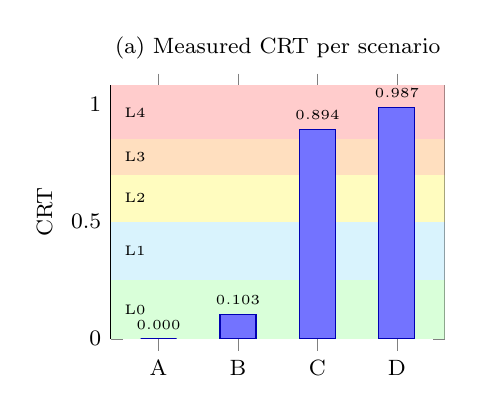
\begin{tikzpicture}
\begin{axis}[
    ybar, width=0.48\linewidth, height=4.8cm,
    ylabel={CRT}, ymin=0, ymax=1.08,
    xtick={1,2,3,4}, xticklabels={A, B, C, D},
    xmin=0.4, xmax=4.6, bar width=13pt,
    nodes near coords={\pgfmathprintnumber[fixed, fixed zerofill, precision=3]{\pgfplotspointmeta}},
    every node near coord/.append style={font=\tiny},
    tick label style={font=\footnotesize}, label style={font=\footnotesize},
    title={\footnotesize (a) Measured CRT per scenario}]
\fill[green!15] (axis cs:0.4,0) rectangle (axis cs:4.6,0.25);
\fill[cyan!15] (axis cs:0.4,0.25) rectangle (axis cs:4.6,0.50);
\fill[yellow!25] (axis cs:0.4,0.50) rectangle (axis cs:4.6,0.70);
\fill[orange!25] (axis cs:0.4,0.70) rectangle (axis cs:4.6,0.85);
\fill[red!20] (axis cs:0.4,0.85) rectangle (axis cs:4.6,1.08);
\node[font=\tiny, anchor=west] at (axis cs:0.45,0.125) {L0};
\node[font=\tiny, anchor=west] at (axis cs:0.45,0.375) {L1};
\node[font=\tiny, anchor=west] at (axis cs:0.45,0.60) {L2};
\node[font=\tiny, anchor=west] at (axis cs:0.45,0.775) {L3};
\node[font=\tiny, anchor=west] at (axis cs:0.45,0.965) {L4};
\addplot[fill=blue!55, draw=blue!70!black] coordinates {(1,0.000) (2,0.103) (3,0.894) (4,0.987)};
\end{axis}
\end{tikzpicture}
\hfill
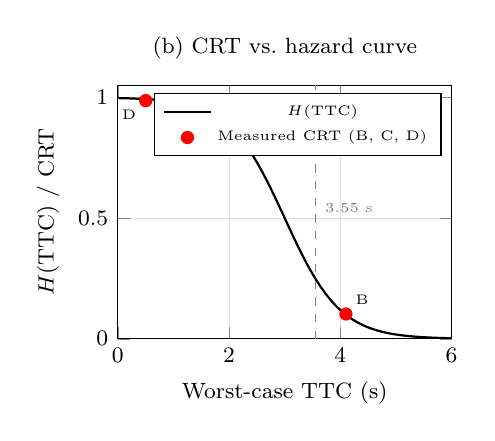
\begin{tikzpicture}
\begin{axis}[
    width=0.48\linewidth, height=4.8cm,
    xlabel={Worst-case TTC (s)}, ylabel={$H(\text{TTC})$ / CRT},
    xmin=0, xmax=6, ymin=0, ymax=1.05, domain=0.01:6, samples=121,
    legend style={font=\tiny}, legend pos=north east,
    tick label style={font=\footnotesize}, label style={font=\footnotesize},
    grid=major, grid style={gray!25},
    title={\footnotesize (b) CRT vs.\ hazard curve}]
\addplot[thick, black] {1/(1+exp((x-3.0)/0.5))};
\addlegendentry{$H(\text{TTC})$}
\addplot[only marks, mark=*, mark size=2.2pt, red] coordinates {(4.1,0.103) (1.9,0.894) (0.5,0.987)};
\addlegendentry{Measured CRT (B, C, D)}
\addplot[thin, gray, dashed] coordinates {(3.55,0) (3.55,1.05)};
\node[font=\tiny, anchor=south west] at (axis cs:4.1,0.103) {B};
\node[font=\tiny, anchor=south west] at (axis cs:1.9,0.894) {C};
\node[font=\tiny, anchor=north east] at (axis cs:0.5,0.987) {D};
\node[font=\tiny, anchor=north west, gray] at (axis cs:3.55,0.6) {3.55 s};
\end{axis}
\end{tikzpicture}
\captionsetup{singlelinecheck = false, format= hang, justification=justified, font=footnotesize, labelsep=space}
\caption{Demo scenarios: (a) CRT values and intervention bands; (b) CRT vs.\ hazard curve.}
\label{fig_scenarios}
\end{figure}

\subsection{Comparison with State-of-the-Art Methods}
Because other methods tackle different goals (like pure trajectory forecasting or offline testing), direct accuracy comparisons on the same data were not possible. Table~\ref{table_comparison} summarizes capability differences based on published papers.

\begin{table}[H]
\caption{Capability comparison with related methods, based on the descriptions in the original papers. Latency is given only for PC-CSG because the other papers do not report it on comparable hardware.}
\centering
\label{table_comparison}
\adjustbox{max width=\linewidth}{
\begin{tabular}{l|c|c|c|c|c|l}
\hline
\textbf{Method} & \textbf{Venue / Year} & \textbf{Counterfactual Hypotheses} & \textbf{Physics Check} & \textbf{Interaction Structure} & \textbf{Risk $\rightarrow$ Action} & \textbf{Setting} \\
\hline
TTC-only baseline & -- & No & No & No & Binary & Online, reactive \\
CRiTIC \cite{ahmadi2025critic} & ICRA 2025 & No & No & Causal gating & No & Online prediction \\
CICR \cite{han2025cicr} & J. Imaging 2025 & Yes (front-door) & No & Social context & No & Prediction \\
Liao et al. \cite{liao2024physics} & IJCAI 2024 & No & Bicycle model & Interaction encoder & No & Prediction \\
TPK \cite{baden2025tpk} & IV 2025 & No & Kinematic layer & Interaction priors & No & Prediction \\
CounterScene \cite{jing2026counterscene} & arXiv 2026 & Yes (causal agent) & No & Causal interaction graph & No & Offline testing \\
STRAP \cite{ning2025strap} & ITSC 2025 & No & No & Risk-field attention & No & Prediction \\
\hline
\textbf{PC-CSG (ours)} & -- & \textbf{Yes (6 modes)} & \textbf{PIKV (6 checks)} & \textbf{Scene graph} & \textbf{5 levels} & \textbf{Online, 6.68~ms} \\
\hline
\end{tabular}
}
\end{table}

As shown in Table~\ref{table_comparison}, existing models each solve only part of the problem. CRiTIC \cite{ahmadi2025critic} focuses on which agents matter, CICR \cite{han2025cicr} and CounterScene \cite{jing2026counterscene} generate counterfactual futures, and Liao et al. \cite{liao2024physics} and TPK \cite{baden2025tpk} make forecasts kinematically feasible. None of them turns physically checked counterfactual risk into graded driver-assistance actions in the perception loop. We see this combination, together with 6.68~ms per frame on a laptop GPU, as the main practical value of PC-CSG. We do not claim better forecasting accuracy than these methods, since we did not measure it.

\section{Conclusion and future scope} \label{section5}
In this paper we presented PC-CSG, a pipeline that adds counterfactual what-if reasoning to the perception loop of an autonomous vehicle and keeps it physically grounded. A scene graph with CPA-based TTC and hazard weights picks the critical agents, CSGA generates and scores six counterfactual hypotheses for each of them, a kinematic bicycle model rolls them out, and PIKV removes the ones that break the friction circle or other vehicle limits before they reach the Counterfactual Risk Tensor. We proved that PIKV removes every friction-violating hypothesis from the risk score, that the physics layers do not depend on the reference frame, that PIKV can never add false alarms, and that the risk score escalates monotonically as the TTC decreases. The 372,068-parameter model runs in 6.68~ms (149.7~FPS) on an RTX 3050 Laptop GPU. PIKV rejected 46.0\% of 678 real hypotheses, and on our validation split PC-CSG reached 100.0\% accuracy with 0.0\% FPR, compared with 94.2\% accuracy and 100.0\% FPR for a reactive TTC-only baseline.

We also found clear limitations: the validation split is small and imbalanced and cannot separate our own variants, the causal gate is computed but not yet applied in the attention, the physics loss term gives no gradient, the earliest warning is still bounded by the TTC gate (about 3.55~s for Level~1), and we could not yet measure a reliable lead time. Fixing these is our first priority. Beyond that, we see two directions for future work:
\begin{enumerate}
    \item \textbf{Multi-modal counterfactual fusion:} Extending CSGA to reason jointly over camera, LiDAR and radar tracks, and evaluating it on nuScenes \cite{caesar2020nuscenes} and Waymo Open \cite{sun2020waymo}, so that counterfactual hypotheses stay reliable when one sensor degrades (rain, glare, night).
    \item \textbf{V2X cooperative counterfactual graphs:} Sharing scene graphs and CRT values between vehicles and roadside units over Vehicle-to-Everything (V2X) links, so that a vehicle can include agents hidden from its own sensors (for example behind a truck) in its counterfactual reasoning.
\end{enumerate}

\bibliography{mybibfile}

\end{document}
